\documentclass[12pt]{article}

% Figures
\usepackage{graphicx}
\usepackage{wrapfig}
\graphicspath{{../plots/}{../tikz/}{../img/}}
\usepackage[section]{placeins} % require floats to appear in the section they are defined

% fonts and appearance
\usepackage{amsmath, amsfonts, physics, siunitx, fleqn, nicefrac}
\usepackage[american]{babel} 
\usepackage[T1]{fontenc} % improved font encoding
\usepackage[ttscale=0.8]{libertine}

% page size and margins
\usepackage{geometry}
\geometry{letterpaper,top=1in, bottom=1in, left=0.5in, right=2in}

% footer
\usepackage{fancyhdr}
\usepackage{lastpage}
\usepackage[en-US]{datetime2}
\fancyhf{}
\fancyhead[L]{DRAFT IN PROGRESS -- Doss-Gollin \& Keller}
\fancyhead[R]{\DTMnow}
\fancyfoot[R]{page~\thepage~of~\pageref{LastPage}}
\pagestyle{fancy}

% TO DO NOTES
\usepackage{xcolor} % list of colors at https://en.wikibooks.org/wiki/LaTeX/Colors
\definecolor{giallo}{HTML}{F0BC42} % https://teamcolorcodes.com/a-s-roma-color-codes/
\definecolor{rosso}{HTML}{8E1F2F}
\definecolor{grigio}{HTML}{CACACC}
\definecolor{nero}{HTML}{000000}
\usepackage[textsize=scriptsize]{todonotes}
\setlength{\marginparwidth}{1.5in}
\newcommand{\james}[1]{\todo[color=giallo, textcolor=nero]{\textbf{ATTN James:~}#1}} % if desired create a custom command for each author
\newcommand{\klaus}[1]{\todo[color=rosso, textcolor=grigio]{\textbf{ATTN Klaus:~}#1}}

% better tables
\usepackage{booktabs}
\usepackage{array}
\newcommand{\PreserveBackslash}[1]{\let\temp=\\#1\let\\=\temp}
\newcolumntype{C}[1]{>{\PreserveBackslash\centering}p{#1}}
\newcolumntype{R}[1]{>{\PreserveBackslash\raggedleft}p{#1}}
\newcolumntype{L}[1]{>{\PreserveBackslash\raggedright}p{#1}}

% better lists
\usepackage[inline]{enumitem}
\setlist{nosep}

% authors
\usepackage{authblk}
\title{Which Scenario Should We Design For? Insights from House Elevation on the Multiple PDF Problem}
\author[1]{James Doss-Gollin}
\author[2,3,4]{Klaus Keller}
\affil[1]{Department of Civil and Environmental Engineering, Rice University}
\affil[2]{Department of Geosciences, the Pennsylvania State University}
\affil[3]{Earth and Environmental Systems Institute, the Pennsylvania State University}
\affil[4]{Thayer School of Engineering, Dartmouth College}
\renewcommand*{\Affilfont}{\normalsize\normalfont}

% ACRONYMS
\usepackage[acronym,nopostdot,nonumberlist,shortcuts,]{glossaries}
\newacronym{bdt}{BDT}{Bayesian decision theory}
\newacronym{bfe}{BFE}{base flood elevation}
\newacronym{fema}{FEMA}{the Federal Emergency Management Agency}
\newacronym{gcm}{GCM}{general circulation model}
\newacronym{lsl}{LSL}{local mean sea level}
\newacronym{mcmc}{MCMC}{Markov Chain Monte Carlo}
\newacronym{mordm}{MORDM}{multiobjective \gls{rdm}}
\newacronym{pdf}{PDF}{probability density function}
\newacronym{rcp}{RCP}{representative concentration pathway}
\newacronym{rslr}{RSLR}{relative sea level rise}
\newacronym{rdm}{RDM}{robust decision making}
\newacronym[plural=SOWs,descriptionplural=states of the world]{sow}{SOW}{state of the world}
\newacronym{tc}{TC}{tropical cyclone}

\usepackage{xspace}
\makeatletter
\DeclareRobustCommand\onedot{\futurelet\@let@token\@onedot}
\def\@onedot{\ifx\@let@token.\else.\null\fi\xspace}
\newcommand{\usd}[1]{\SI{#1}[\$]{}}
\def\eg{\emph{e.g}\onedot} \def\Eg{\emph{E.g}\onedot}
\def\ie{\emph{i.e}\onedot} \def\Ie{\emph{I.e}\onedot}
\def\etc{\emph{etc}\onedot} \def\vs{\emph{vs}\onedot}

% use biblatex
\usepackage{csquotes}
\usepackage[
  backend=biber,
  doi=true,
  url=false,
  isbn=false,
  style=authoryear-comp,
  natbib=true,
  backref=false,
  maxbibnames=10,
  maxcitenames=2,
  uniquename=false,
  uniquelist=false,
  sorting=nyt,
]{biblatex}
\renewbibmacro{in:}{}
\AtEveryBibitem{\clearfield{month}\clearfield{day}\clearfield{pages}\clearlist{language}}
%\addbibresource{../_bibliography/library.bib}
\addbibresource{library.bib}

% load this last
\usepackage[hidelinks]{hyperref}
\usepackage{cleveref}

% up to 1250 words
\begin{document}
\maketitle
\thispagestyle{empty}

\begin{abstract}
    Many homeowners in the coastal zone elevate their houses to manage flood risk.
    Federal guidance for this decision relies on floodplain maps that are silent on projected future changes and neglect the deep and dynamic uncertainties surrounding the projected hazards.
    This uncertainty poses challenges for the design of decision-support systems.\james{If this is about RDM then let's lead with that.}

    Many methods for decision making under deep uncertainty first evaluate candidate decisions over many plausible states of the world, then aggregate performance over these possible futures.
    Through a didactic case study of determining how high to elevate a single home in Norfolk, VA, we demonstrate that the common practice of weighting all scenarios equally in this aggregation creates a tension between (a) fully exploring the parameter space, including unlikely regions, and (b) accurately representing available scientific knowledge.
    We introduce an approach to bridge this divide through a computationally efficient method that weights each state of the world based on a probability distribution over possible futures.
    Since the distribution of deeply uncertain variables is necessarily subjective, we turn to frameworks for model critique from applied Bayesian statistics to compare and contrast different modeling assumptions.
    This approach can help to improve decision-making by facilitating iterative and collaborative model improvement.
\end{abstract}

\section*{Front Matter}

\subsection*{Submission Plan}
We should revisit this!
\begin{enumerate}
    \item Earth's Future
    \item Climatic Change
    \item IOP Environmental Research: Infrastructure and Sustainability (new journal)
    \item Risk analysis
\end{enumerate}
\subsection*{Internal peer review}
\begin{enumerate}
    \item Vivek
    \item Courtney
    \item Sanjib
    \item Kelsey to replicate code
\end{enumerate}

\clearpage
\section{Introduction}

\paragraph{Why this problem is important}
Since infrastructure built today is likely to persist for several decades, infrastructure designs must take into account the stresses that a project is likely to face far into the future.
On the one hand, overly optimistic assumptions of future risk can lead to unacceptably high risk of failure in the future if additional investments are not made.
For example, a failure to prepare Texas's interconnected natural gas, electricity, and water systems for temperatures that had been observed in the past 30 years caused cascading failures with disparate impacts \citep{doss-gollin_txtreme:2021,busby_cascadingrisks:2021}.
On the other, unless opportunity costs are negligible, designing for a too-pessimistic scenario can contribute to maladptation by limiting resource availability in the future.
For example, \ldots\james{add an example of a maladaptive megaproject -- look to sustainability science or the arguments in \citet{ansar_bigisfragile:2017}.}

\paragraph{Set up the ``Multiple PDF Problem''}
While classical utility- or regret-based frameworks offer a structure for weighing these risks, they are not designed to handle uncertainties that are \emph{deep} in the sense that stakeholders may not agree upon their probabilities \citep{lempert_complex:2002} or \emph{irreducible} in the sense that there is not an objective truth that better models and data can identify \citep{DossGollin:2019}.\footnote{Unless we believe everything is pre-determined, in which case why bother with climate adaptation\ldots}
Examples of such uncertainties include how much greenhouse gasses humans will emit in the future or whether the U.S. federal government will continue to subsidize flood insurance for homeowners.\james{Add some references}
In response, a wide range of fields have developed scenario-based methods\ldots.\klaus{Which arguments in \citet{savage:1954} did you think should be cited here?}
This leads to the ``Multiple PDF Problem'' \citep{sharma_rcp:2021}\ldots.
A key question, then, facing the designers, builders, regulators, owners, and users of built facilities is \emph{to which scenario should infrastructure be designed?}

\paragraph{Set up house elevation as an example}
One example is building codes and guidelines\ldots.
Prior studies have found that floodproofing and building-scale vulnerability reduction measures, including house elevation, can effectively reduce local flood damages in many contexts \citep{demoel_reducing:2014,deruig_building:2020,kreibich_building:2005,slotter_floodproofing:2020,Rozer:2016dn,mobley_mitigation:2020,aerts_cost:2018}.
Official guidance for homeowners, notably from \gls{fema}, recommends elevating to the \gls{bfe} (typically the \SI{100}{year} flood) plus a freeboard \citep{fema_retrofitting:2014,asce_24-14:2015,fema_retrofitting:2014} but recent suggests scope for improvement.
For example, \citet{xian_elevation:2017} used a cost-benefit analysis to demonstrate that tailoring recommendations to the inital elevation of a structure can reduce expected costs.
\citet{zarekarizi_suboptimal:2020} show that neglecting uncertainty in discount rate, house lifespan, flood risk, and depth-damage curves can lead to maladaptation.
Yet these studies are silent on the question of how nonstationary flood hazard should factor into this decision.

\paragraph{Nonstationarity motivates the case study}
Nonstationarity is particularly relevant in coastal communities where \gls{rslr} is expected to drive future flood risk.
As a didactic case study, we consider the problem of how high a homeowner should elevate their structure to mitigate future flood losses, illustrated in \cref{fig:house-sketch},\james{Need to revisit this picture} given stochastic flood peaks and deeply uncertain \gls{rslr}.
\Gls{rslr} is driven mainly by physical processes like (\ldots, West Antarctic Ice Sheet, \ldots\klaus{You wrote something here that I can't read -- I see something that looks like ICM. I assume Tony and Kelsey papers are relevant as well?}) \citep{kopp_probabilistic:2014,kopp_evolving:2017}.
Two key uncertainties identified by previous studies are
\begin{enumerate*}[label=(\roman*)]
    \item which emissions pathway (\eg, \gls{rcp} scenario) will we experience and
    \item how will polar ice sheets respond to warming \citep{wong_brick0.2:2017,ruckert_coastal:2019,wong_nola:2017,deconto_antarctica:2016}.
\end{enumerate*}
Simulations of \gls{rslr} are available to decision makers grouped by \gls{rcp} scenario and model structure.
For a given combination of \gls{rcp} scenario and model, results are typically presented and interpreted as probabilistic, but this is not the same as giving decision-makers a single \gls{pdf}.
This is the ``Multiple \gls{pdf} Problem'' described in, \eg, \citet{sharma_rcp:2021}.
Thus, \emph{which scenario/\gls{pdf} should we design for?}

\paragraph{Needs work}
Lacking a crystal ball capable of telling us precisely which \gls{pdf} we need to design for, we have to consider several as plausible.
Any decision will perform differently in different scenarios.
There is no objective answer to this question.
Since we can't be ojectively correct, we might as well be transparent and make our assumptions explicit (and subject to critique) rather than implicit.

\paragraph{Roadmap}
We first present a general framework for\ldots.
We then illustrate this method through a didactic case study of deciding if, and how high, to elevate a single house in Norfolk, VA.

\begin{figure}
    \centering
    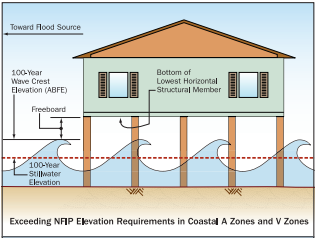
\includegraphics[height=2in]{uconn-elevateA}
    \caption{
        Conceptual sketch illustrating the path from historical data to FEMA's guidance.
        This figure \emph{needs to be revised} (KATERINA?) to have three panels, of which this is the third.
        (a): A time series of historical floods.
        (b): A \gls{pdf} of the flood peak.
        (c): as shown, but with waves eliminated.
        This sketch figure is from \citet{patten_elevate:2016}.
    }\label{fig:house-sketch}
\end{figure}

\section{Decision framework}\label{sec:framework}

In this section we present a general framework for decision making under deep uncertainty.
We begin with terms and definitions that are broadly consistent with common adaptive frameworks\james{add refs}\klaus{did I read this right?}.
In \cref{sec:methods-weight} we present a Bayesian model for weighting \glspl{sow}.
In \cref{sec:methods-iterative} we discuss how this framework can be integrated into frameworks for iterative engagement with experts and stakeholders to expand and frame the model.

\begin{figure}
    \centering
    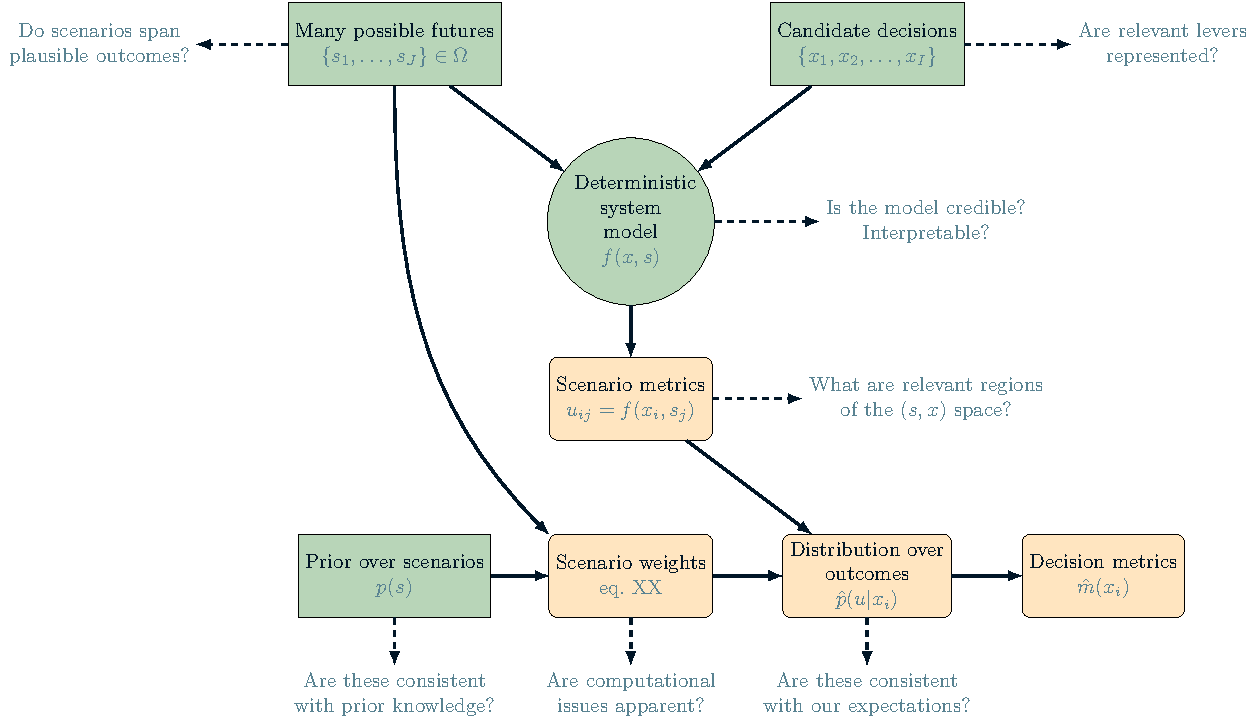
\includegraphics[width=\textwidth, height=4.5in, keepaspectratio=true]{conceptual.pdf}
    \caption{
        Schematic of our decision support framework.
        Nodes in green are modeling choices that the modeler must make while those in yellow are computed quantities.
        Teal text illustrates a non-exhaustive set of opportunities to perform model checks and/or engage with stakeholders to iterate on design of the decision support system.
        Feedbacks between these questions and the green nodes are omitted for clarity.
        Our approach could be extended by coupling the evaluation framework to an optimization or policy search tool that updates the candidate decisions.
        This approach could also be extended to a stochastic system model.
    }\label{fig:framework}
\end{figure}

We start by modeling the performance of a decision $x \in \mathcal{X}$.
Outcomes depend both on the decision and on a state of the world $s \in \Omega$ that describes all relevant uncertainties.
To model outcomes $u \in \mathcal{U}$, we use a system model $f: \mathcal{X}, \Omega \rightarrow \mathcal{U}$ \citep[we generally follow the notation of][]{mcphail_robustness:2019} which we assume to be deterministic.
If $f$ is a stochastic function, we can define its metrics in terms of expectations, \eg $u_{ij} = \mathbb{E}\qty[u | x=x_i, s=s_j]$, which can be approximated through techniques like Monte Carlo sampling.

The literature on decision making under deep uncertainty \citep[see][for a review]{marchau:2019} emphasizes the importance of using system models like $f$ in an exploratory context by sampling widely from plausible futures $s \in \Omega$ and studying their implications \citep{bankes:1993,lempert_shaping:2003,kwakkel:2019,lamontagne_discovery:2018}.
This is often described as ``bottom-up'' modeling \citep{Brown:2012kb} and has parallels to model-based stress tests and vulnerability assessments.

Given our system model $f$ and a sampling of $J$ possible states of the world $s_1, s_2, \ldots, s_J$, we can calculate a set of \emph{\gls{sow} metrics} $u_{ij}$ that tell us ``how will decision $x_i$ perform under state of the world $s_j$'' for many $s_j$, and one or more $x_i$.
For an apples to apples comparison of how different decisions perform on the $j$th \gls{sow}, we can directly compare $u_{1j}, u_{2j}, \ldots, u_{Ij}$.
However, if we wish to compare the performance of two or more decisions across \emph{all} scenarios, we will need some way of aggregating the \gls{sow} metrics into \emph{decision metrics} $m_1, m_2, \ldots, m_I$ such that for every $x_i$ there is a single (scalar or vector) $m_i$.\footnote{I think the link back to our original motivation -- the multiple PDF problem}

\citet{mcphail_robustness:2019} split the problem of aggregating \gls{sow} metrics into decision metrics into two steps: ``subsetting'' (\eg, single value, all values, subset of values) and ``metric calculation'' (\eg, mean, variance, skew, kurtosis).\klaus{You say something about see discussion in \citet{mcinerney_robust:2012} -- please elaborate}
We generalize this to
\begin{equation}
    m_i = g(\qty{u_{i1}, u_{i2}, \ldots, u_{iJ}}, \qty{w_1, w_2, \ldots, w_J}),
\end{equation}
where $g$ is an \emph{aggregating function} describing the ``metric calculation'' step and the $w_j$ describe weights given to each \gls{sow}.
A optional, but likely useful, interpretation of the weighted samples $\qty{w_j, u_{ij} \forall j=1, \ldots, J}$ is an empirical \gls{pdf}, in which case $g$ maps a \gls{pdf} of future outcomes to the metrics $m_i$.\footnote{perhaps this belongs in the Discussion}
This is a flexible framework; \cref{tab:literature-weighting} shows some methods for robust decision making from the literature using our notation.\james{Add some references to the table}

\begin{table}
    \centering
    \footnotesize
    \begin{tabular}{llll}
        \toprule
        Citation        & Explanation                     & $w_j$                                                                             & $g(u, w)$          \\
        \midrule
        Many            & All $s_j$ are equally plausible & $w_j = \nicefrac{1}{J}$                                                           & any                \\
        Many            & Worst case                      & $w_j = \begin{cases}1 & u_{ij} = \min_{j'} u_{ij'} \\ 0 & \text{else}\end{cases}$ & $u$                \\
        TBD             & Average over \glspl{sow}        & $w_j = \nicefrac{1}{J}$                                                           & $\sum_j w_j u_{j}$ \\
        Characklis/Reed & 95th percentile                 & $w_j = \nicefrac{1}{J}$                                                           & weighted quantile  \\
        \bottomrule
    \end{tabular}
    \caption{
        A non-exhaustive summary of methods for setting $w_j$ and $g$ from the literature.
        (\emph{What other examples should we add?})
    }\label{tab:literature-weighting}
\end{table}

In the next section we propose an alternative scheme for weighting scenarios.

\paragraph{To think  about}
I have two flavors of this idea presented here!
\Cref{fig:framework}\james{Updates for \cref{fig:framework}: Don't need to say here that $f$ is deterministic. Larger text and darker color for questions. Rename $p(s)$ as ``prior over parameters and model structures''} takes a more Bayesian focus: the goal is to reason about properties of the \emph{distribution} over outcomes $p(u | x=x_i)$.
The text follows \citet{mcphail_robustness:2019} more.
I'm not sure which is easier to understand.

\subsection{Weighting \glsentryplural{sow}}\label{sec:methods-weight}

If the common practice of weighting all scenarios equally is applied ($w_j \propto 1$ in \cref{tab:literature-weighting}), a tension emerges: we want to \emph{explore} highly unlikely but theoretically possible trajectories to understand their consequences, but we don't want extremely unlikely scenarios to dominate our decision.

Some aims:
\begin{enumerate}
    \item Assumptions should be as transparent and visible as possible to facilitate critique and dialogue\klaus{I moved this up}
    \item We should be invariant to the parameterization of $s$ -- if we sample population uniformly from 1 million to 10 million or $\log_{10}$ population uniformly from \num6 to 7, we should get the same answer
    \item We should be invariant to the sampling of $s$:
          \begin{enumerate}
              \item if we include scientifically interesting but extremely low-probability scenarios (\eg, if someone created \gls{rcp} 45), our esimtates of $m_i$ should not change meaningfully.\james{Explain why}
              \item if we include nearly redundant scenarios (\eg, if we are studying \gls{rcp} 2.6, 4.5, 6.0, and 8.5 and we then add results from a \gls{rcp} 6.01 experiment), our estimates of $m_i$ should not change meaningfully.\james{Explain why}
          \end{enumerate}
\end{enumerate}
We can do this with probability if we have a target distribution $p(s)$.
We return to the question of how to choose this in \cref{sec:methods-prior}.

\subsection{Melding prior over \glsentryplural{sow}}\label{sec:methods-prior}

Often (including in the case study described in \cref{sec:case}) our \glspl{sow} are the outputs of complicated model chains.
To set our prior $p(s)$ we might like to incorporate prior external knowledge about both the

\subsection{Opportunities for iterative model expansion}\label{sec:methods-iterative}

\paragraph{Robustness checks}
The computationally expensive piece is computing the $u_{ij}$.
Once you do that, you can look at several $p(\Omega)$ and compute the $m_i$ multiple times.

\paragraph{Links to DMDU Methods}
You can use scenario discovery on the $(x_i, \mu_{ij}$).
(Others to note?)

\paragraph{Bayesian model checks}
Let's just cite \citet{gelman_workflow:2020} and \citet{gabry_visualization:2019} and point out that you can and should conduct sample-based checks on your prior $p(\Omega)$ and your posterior $p(u | x=x_i)$.\footnote{See discussion above about whether we want to emphasize that we are treating this as a posterior or not}

\section{Case study: house elevation}\label{sec:case}

We start with a bare-bones version of the \citet{zarekarizi_suboptimal:2020} model.
For interpretability, we fix the discount rate, house lifetime, and depth-damage curve to illustrate how our framework can be used to model nonstationary flood risk.
Real-world decision makers should consider additional uncertainties and stakeholder-identified metrics.

\begin{figure}
    \centering
    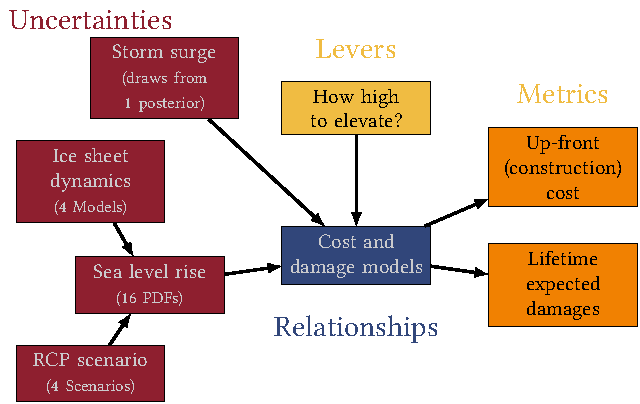
\includegraphics[height=2.5in, width=0.6\textwidth, keepaspectratio=true]{xlrm}
    \caption{
        Diagram showing uncertainties ($X$; red), levers ($L$; yellow), system relationships ($R$; gray), and metrics ($M$; blue).
    }\label{fig:xlrm}
\end{figure}

\subsection{Scenarios}

Coastal floods are often decomposed into changes in local sea level \citep{kopp_evolving:2017,kopp_probabilistic:2014,wong_brick0.2:2017} plus storm surge \citep{garner_slrise:2018,cagigal_emulator:2020,rueda_surge:2016}.
We neglect waves and hydrodynamics for simplicity.

\gls{rslr}:
\begin{enumerate}
    \item We have 2 models of ice sheet dynamics (3? Vivek and Tony are trying to tell me what models the data from \citet{ruckert_coastal:2019} actually comes from)
    \item We have 4 \gls{rcp} scenario
    \item We use the BRICK model \citep{wong_brick0.2:2017} simulations from \citet{ruckert_coastal:2019} to define $J$ \glspl{sow}.
\end{enumerate}
Storm surge:
\begin{enumerate}
    \item We have a $N$ year observational record
    \item We separate out storm surge from the background trend in some standard way
    \item We model storm surge as a stationary GEV model
    \item We place a prior on the return level (data space) rather than a prior on the parameters themselves (except the shape parameter -- we put a restrictive prior for it to be positive)\james{arguably we should stick to boring priors here -- the question being whether it's better to say we use iterative checks to improve the priors, or whether we want to keep things simple}
    \item We draw $K$ sets of parameters $\qty(\mu_k, \sigma_k, \xi_k)$
\end{enumerate}
Thus a \gls{sow} is defined just an 81 year time series of \gls{lsl}.
We will see what we do with the $K$ draws of storm surge parameters shortly.
\begin{figure}
    \caption{
        INSERT HERE: figure showing time series of observed surge and \gls{lsl} with notable storms indicated, as well as projections of future \gls{lsl} under all eight models (two BRICK, four \gls{rcp})
    }
\end{figure}

\subsection{Decisions}

We consider only one lever: how high to elevate the house today.
This is the same lever considered in \citet{zarekarizi_suboptimal:2020}

\subsection{Metrics}

Three scenario metrics $u$:
\begin{enumerate}
    \item Construction cost
    \item Discounted expected flood damages
    \item Total cost (construction plus flood)
\end{enumerate}
The decision metrics $m$ are just the expected value of $u$.

\subsection{A simplified didactic system model}

\begin{enumerate}
    \item Costs of elevating the house are the same as \citet{zarekarizi_suboptimal:2020}
    \item Depth-damage: use HAZUS model from \citet{zarekarizi_suboptimal:2020}
    \item Discount: fix at some appropriate rate (2\%?)
    \item House lifetime: fix at some reasonable amount (80 years)
\end{enumerate}

Recall that we have $K$ simulations of the storm surge parameters.
For each year of each \gls{sow} we would like to estimate the expected value of the convolution of hazard (storm surge plus \gls{lsl}) with fragility (depth-damage).
A simple algorithm to estimate this is, for each \gls{pdf} of storm surge $k \in 1, \ldots, K$, to draw $N$ Monte Carlo sample values of storm surge, calculate the damage associated with each, and take the expectation with respect to $N$.
Then, take the expectation again with respect to the $K$ storm surge \glspl{pdf}.
Since this is computationally expensive, we build an emulator that estimates expected damage as a function of mean sea level only by fitting a spline to the result of systematically calculating expected damages for different values of \gls{lsl}.\footnote{A supplemental figure would be good here. This is probably a bit dense of a discussion.}

\begin{figure}
    \caption{
        INSERT HERE: figure showing the convolution of storm surge hazard through the depth-damage function.
        We fix \gls{lsl} constant but have many \glspl{pdf} of \gls{lsl}.
        This is the ``hazard, damage, risk'' graph that Klaus has sketched.
    }
\end{figure}

\subsection{Belief model}

\paragraph{Prior on outputs only}
Following \citet{garner_slrise:2018}, \citet{oddo_coastal:2017}, and \citet{lempert_slr:2012} we place a prior on \gls{rslr} in 2100.\klaus{You suggest looking at another paper. Are you referring to this?\\\fullcite{sriver_sealevel:2018}}

\paragraph{Prior on inputs only}
Alternatively, we can place a prior over scenarios.
Let's say that we think that emissions forcing in 2100 is has some distribution.
This means we are placing a weight over \gls{rcp} scenarios.
We can assume both BRICK models are equally likely.

\paragraph{Melding}
We can do cool stuff with Bayesian melding \citep{poole_melding:2000,sevcikova_melding:2007}.
This combines the prior over inputs and outputs geometrically.
\begin{equation}\label{eq:melding}
    \text{melding equation here}
\end{equation}
This lets us express information about some inputs being more or less likely than others, and also some outputs being more or less likely than others.
THIS IS USEFUL because often we would like to incorporate relevant knowledge from many different sources on both inputs and outputs (\eg, IPCC reports, National Climate Assessments, \etc).

\paragraph{Implementation}
Code will be available on GitHub.
We use the Julia programming language.

\section{Results}\label{sec:results}

We will need a figure or two showing our prior and posterior checks, as well as some results.
Results should show the tradeoff between cost and damage under different assumptions.

\section{Discussion}

Most fundamentally, we are thinking about robustness a bit differently than usual.
The typical way that the DMDU literature thinks about it is robustness to a \gls{sow}.
We are thinking about robustness to different modeling structures and assumptions.
This has links to the ``rival framings'' literature that Pat has been working on.
Given a subjective prior $p(s)$, I can compute expectations of the decision metrics $m$; if there are a lot of decisions, I can start to sketch out the tradeoff curves as shown in figures XXXX (in \cref{sec:results}).

\begin{enumerate}
    \item Links to DMDU literature
          \begin{enumerate}
              \item We should also cite \citet{quinn_exploratory:2020}, which makes the point that it matters how you sample \glspl{sow}.
              \item Exploratory modeling can demonstrate the existence of particular outcomes, generate hypotheses, build qualitative insight, and identify scenarios worthy of further study \citep[see][]{bankes:1993}.
              \item You can do scenario discovery
              \item We are in effect calculating robustness metrics \citep{mcphail_robustness:2019,herman:2015}
          \end{enumerate}
    \item Philosophy of Bayesian stats / decision making
          \begin{enumerate}
              \item The observation that many of these mechanisms cannot be represented by a single objective \gls{pdf} has motivated many criticisms of the application of \gls{bdt} to planning problems.
                    Yet \gls{bdt} was conceived as a calculus for reasoning rather than for identifying objective truth; \citeauthor{definetti_probability:1972} often said that ``probability does not exist'' \citeyear{definetti_probability:1972}.
                    \citet{savage:1954} and \citet{ramsey_probability:2016}, among others, also viewed probability as ``subjective,'' representing the state of belief of the decision-maker.
                    The famous phrase ``all models are wrong, but some are useful'' \citep[generally attributed to][]{box:1976} also suggests that probability distributions and predictions ought to be viewed subjectively.
                    More recent discussions of Bayesian philosophy \citep{jaynes_probability:2003,McElreath:2016vu,Gelman:2014tc,bernardo_bayesian:1994} also emphasize a philosophical view of probability as a language with which to reason about the unknown rather than a statement of objective truth \citep[see][for a thorough discussion of Bayesian philosophy]{gelman_philosophy:2013}.\klaus{Am I reading right that you say ``maybve have this in intro to motivate the analysis?''}
                    Although the true data generating process is not known and inference should not be represented as objective truth, probability gives a transparent and consistent language for reasoning about uncertainty.
                    Since modeling assumptions cannot overcome epistemic uncertainty, even with better models and more data, we draw from the literature on statistical model selection in the $\mathcal{M}$-open setting, which provides a theoretical background for choosing between models when the true data generating process is not among the models considered \citep[see][]{Piironen:2017eh}.
                    Often, combining inferences from multiple models is more effective than seeking a single ``best'' model \citep{Yao:2018bu}.
                    More fundamentally, this literature emphasizes the importance of iteratively building models, simulating the consequences of those models, and critiquing them \citep{gelman_workflow:2020}.
                    Since, by definition, models are not ``true,'' this iterative workflow aims to identify models that are useful and promote a dialog amongst stakeholders \citep{gelman_philosophy:2013}\footnote{this paragraph is copied from my dissertation, needs to be re-worked!}
          \end{enumerate}
    \item There are interesting links to Bayesian model averaging
          \begin{enumerate}
              \item Lots of examples to cite if we want
              \item I'm partial to something like stacking \citep{Yao:2018bu}
              \item The main difference is we are using only the prior to average the models!
          \end{enumerate}
    \item Limitations of the case study
          \begin{enumerate}
              \item Objectives: real people might care about uncertainty (risk aversion), probability of experiencing flooding at all (disruptions are hard to quantify), usable space created under the house, and more
              \item More uncertainty (damage functions, cost of construction, lifespan, discount rate, \etc)
              \item Better data on cost of elevation and depth-damage
              \item Robustness: ptimize separately for different kinds of house structures and locations
              \item Timing
          \end{enumerate}
    \item Limitations of the method
          \begin{enumerate}
              \item Our prior $p(s)$ is limited -- we are just using \gls{lsl} in 2100 but we could be looking at more parameters of it including rate of change, \etc
              \item We neglect true ignorance \citep{knight_risk:1921}.
              \item The real world is in a state of ``unknown unknowns'' \citep[level 5 as defined in][fig.~1]{walker_deep:2013} so trying to represent \emph{all} uncertainty is futile; we must make subjective modeling choices and assumptions about what is most important
          \end{enumerate}
    \item The benefits of this approach:
          \begin{enumerate}
              \item A goal is to make -- intrinsically flawed and subjective -- modeling choices as transparent as possible. Since we can't be right, we should make it as easy as possible for others to understand and critique our assumptions\james{Focus on this!}
              \item Because of how we weight realizations of the future, you can apply a different weighting function and immediately assess performance. Thus qualitative and quantitative sensitivity analyses are simple.
              \item Of course the choice of $p(\mathcal{Z})$ is subjective, but so is every other aspect of how we frame the problem. Modeling is intrinsically subjective. The idea of embracing subjective choices -- and making them explicit and open to critique -- draws heavily from philosophies of iterative workflow in statistics \citep{box:1976,gelman_workflow:2020,gelman_philosophy:2013}.
              \item This approach can be used in a multiobjective context and is an alternative way to measure robustness in \gls{rdm} and \gls{mordm}
          \end{enumerate}
    \item This approach can be used in many other contexts
          \begin{enumerate}
              \item Direct
                    \begin{enumerate}
                        \item Stormwater management \citep{sharma_rcp:2021,lopez-cantu:2018}
                        \item Levee heightening \citep{garner_slrise:2018,oddo_coastal:2017,vandantzig_dike:1956}
                    \end{enumerate}
              \item Indirect
                    \begin{enumerate}
                        \item Lots of economic models like social cost of carbon or effect of policy on metrics of interest make assumptions about deep uncertainties!
                        \item Model structure uncertainties
                    \end{enumerate}
          \end{enumerate}
\end{enumerate}.

\section{Conclusions}

\begin{enumerate}
    \item We started with the problem of ``which scenario should we design to?'' We then devised a cop-out: design to a weighted combination of all the scenarios. (So how should we wight the scenarios? Come up with a model $p(\Omega)$ that tells you.)
    \item There is no objective way to choose $p(\Omega)$ because we don't have data on the future!
    \item We can't get around from choosing $p(\Omega)$ implicitly\footnote{I'm not sure we have demonstrated this rigorously, or whether we want to argue it, but I think there's a way to frame this point that is valid and helpful}
    \item Ultimately, engineering design needs to consider not only how to weight different future scenarios, but also which metrics are important, how risk aversion should be addressed, \etc.
    \item We used a didactic case study to present a toolkit (decision framework, melding priors, prior over return levels) for making transparent and critique-friendly assessments.
\end{enumerate}

\section*{End Matter}

\subsection*{Acknowledgements}

\begin{enumerate}
    \item MARISA\james{details}
    \item PSIRC\james{details}
    \item Rice University (for startup)
    \item Tor Erlend Fjelde for helpful advice on implementing the GEV prior using \texttt{Turing.jl}.
    \item For many journals, a code and data statement will go here.
\end{enumerate}

\subsection*{Author Contributions}

See journal requirements and format

\subsection*{Supplementary Materials}

\begin{enumerate}
    \item Supplementary figures and analysis online
    \item Link to live repository on GitHub
    \item Link to code DOI on Zenodo
\end{enumerate}

\printbibliography
\end{document}
